% Para iniciar una sección debe escribirse
%\section{Nombre de la sección}
% Lo anterior inmediatamente creará la sección y la numerará.

\section*{Objetivos}
\subsection*{Generales}
\begin{itemize}
    \item Diseñar y construir una calculadora capaz de realizar operaciones aritméticas básicas capaz de desplegar la información en formato base 10
\end{itemize}

\subsection*{Específicos}
\begin{itemize}
    \item Diseñar múltiples circuitos combinacionales para obtener un resultado único en conjunto
    \item Implementar un circuito de lógica combinacional capaz de realizar operaciones aritméticas simples utilizando únicamente compuertas lógicas
    \item Optimizar el uso de compuertas mediante técnicas distintas al uso de Mapas de Karnaugh
    \item Contrastar los diseños teóricos con los resultados experimentales de los circuitos implementados físicamente
\end{itemize}

\section{Introducción}

\subsection{Aritmética binaria}
Los dispositivos digitales se basan en operaciones con numeración \emph{base 2} para obtener los resultados, incluso si la interfaz de usuario tuviese otro 
formato (numérico decimal, en base a gráficos o imágenes, etc.). Las operaciones aritméticas en \emph{base 2} cumplen con los mismos teoremas y reglas que se
utilizan en base 10, pero poseen la ventaja de tener más simplificaciones debido a la limitada cantidad de dígitos disponibles. Consulte su libro de
texto\footnote{Mano, Morris. Digital Design, 5th edition} para recapitular lo anteriormente descrito.

% \begin{figure}[H]
%     \centering
%     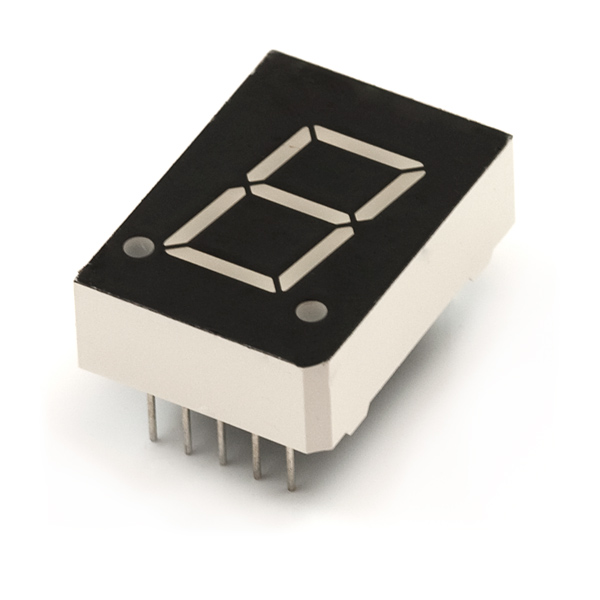
\includegraphics[scale=0.3]{images/7SegmentDisplay.jpg}
%     \caption{Display de 7 segmentos}
%     \label{Fig:SevenSegment}
% \end{figure}


\pagebreak

\section{Desarrollo Experimental}
\subsection{Materiales y Equipo}

Cada grupo debe llevar su material y equipo de trabajo durante las prácticas. Pregunte a su profesor qué \emph{Equipo de Laboratorio} puede ser prestado
de parte del laboratorio de instrumentación. El laboratorio de instrumentación no tiene disponibilidad de ningún elemento de la lista \emph{Materiales}.

\subsubsection*{Materiales}
\begin{itemize}
    \item 1x dip-switch de 7 posiciones (o más)
    \item 7x pulsadores (si no consiguiesen el dip-switch de 4 posiciones)
    \item 1x fuente de alimentación (ver apartado anterior con todas las alternativas)
    \item 2x capacitores electrolíticos de 47 $\mu$F 16V
    \item 2x capacitores cerámicos de 100nF 25V
    \item 6x resistencias de 1 k$\ohm$
    \item 2x LEDs de cualquier color
    \item 1x Display de 7 segmentos de \textbf{ánodo común} de cualquier color
    \item 7x Resistencias $220 \ohm \leq R \leq 1 k\ohm$
    \item 6x metros de alambre para protoboard calibre 22. Compren al menos 2 colores para los 6 metros. \textbf{No usen \emph{UTP}}, aunque eso les quieran vender.
    \item 1x Circuito Integrado 74LS47 (decodificador BCD a Display 7 segmentos ánodo común)
    \item Las compuertas lógicas a utilizar dependen del diseño final de cada grupo (AND, OR, NOT, XOR, NAND, XNOR)
\end{itemize}


\subsubsection*{Equipo de Laboratorio}
\begin{itemize}
    \item 1x Pinzas delgadas
    \item 1x Cortaalambres
    \item 1x Pelador de alambres para calibre 22 (opcional)
    \item 1x Tijeras pequeñas o cortauñas (si no tienen pela alambres)
    \item 1x Protoboard de al menos 2 galletas (puede juntar 2 protoboards de 1 galleta)
    \item 1x Multímetro digital para medir voltaje
\end{itemize}

\subsection{Procedimiento}
\subsubsection{Fuente de alimentación}
Utilice la misma fuente de alimentación que en la Práctica \#1.

\subsubsection{Calculadora básica}
Se debe diseñar una calculadora con entradas a través de una interfaz binaria (dip-switch o pulsadores) que despliegue el resultado de la
operación en un display de 7 segmentos. Las operaciones a realizar son:
\begin{itemize}
    \item Suma 
    \item Resta sin signo
    \item Indicar Overflow/Underflow con un LED
\end{itemize}

\vspace{14pt}

El método de entrada son 2 variables de 3 bits ($A_0, A_1, A_2, B_0, B_1, B_2$) a través de \emph{dip-switch} o pulsadores. Además, debe existir
un interruptor dedicado para seleccionar si la operación a realizar es \emph{suma} o \emph{resta sin signo}.
Debido a que el CI 74LS47 despliega caracteres no alfanuméricos con para valores entre 0x0A y 0x0F, no será necesario hacer ninguna corrección para
mostrar el valor adecuado.






\vspace{14pt}

Por ejemplo: si el año de ingreso fuese \emph{2018}, se le asignaría un índice (posición) a cada dígito como se
muestra en la Tabla \ref{Table:ejemploIndices}.

\begin{table}[H]
    \centering
    \begin{tabular}{|c|c|c|c|c|}
        \hline
        \textbf{Dígito} & 2 & 0 & 1 & 8 \\ \hline
        \textbf{Índice}  & 1 & 2 & 3 & 4 \\ \hline
    \end{tabular}
    \caption{Ejemplo de asignación de índice a cada dígito}
    \label{Table:ejemploIndices}
\end{table}


En otras palabras, el \textbf{índice 2} corresponde al \textbf{dígito 0}; al \textbf{índice 3} le corresponde el \textbf{dígito 1} y de la misma forma para el resto...

\vspace{14 pt}

El objetivo de esta sección será diseñar y construir un circuito que codifique cada uno de los índices (del 1 al 4) al dígito correspondiente en el año a mostrar.
Las salidas deben ser la representación en BCD de cada dígito, asignado al índice de cada entrada.

\vspace{14 pt}

El método de entrada es a través del dip-switch (no olivde las resistencias \emph{pull-down}) de 3 posiciones, en el que el usuairo
selecciona un valor de índice (de 1 a 4) y la salida es el dígito correspondiente al índice,
la cuál se despliega a través de 4 LEDs (siempre con sus resistencias limitadoras de corriente).

\subsubsection*{Importante}
\begin{itemize}
    \item Si el usuario selecciona un índice inválido (0, 5, 6, 7) la salida del circuito debe ser siempre $1111_2$
    \item Tome en cuenta que la salida debe ser de 4 bits, ya que un dígito puede tener un valor entre 0 y 9.
    \item Cada grupo de trabajo puede seleccionar un número a codificar, no necesariamente puede ser un año. El único requisito es que tenga al menos 4 dígitos.
\end{itemize}

\subsection{Interfaz de salida}
En esta sección convertirán la información BCD en un número humanamente amigable: el display de 7 segmentos es la forma más sencilla de lograr
el elemento de salida de la interfaz humano-máquina. Se utilizará un circuito integrado decodificación de BCD a Display para esta tarea.

Por primera vez se le dejará como tarea interpretar una hoja de datos de fabricante, en este caso, para comprender el funcionamiento detallado y
conexionado del 74LS47. Cualquier duda consúltela a su instructor. Consejo: no se enfoque en el diagrama lógico que aparece en la hoja de datos,
utilice mejor la tabla de verdad y las descripciones de cada pin. Las primeras 2 páginas de la hoja de datos contienen toda la información necesaria
para realizar la práctica.

\subsubsection*{Importante}
Recuerde que al trabajar con un display de ánodo común, la activación de un elemento se hace através de un \textbf{0 lógico}. No olvide esto
al estar analizando la tabla de verdad en la hoja de datos del integrado.

\subsubsection{Resistencias de cátodos}
Para limitar la corriente que circula en cada uno de los LED que conforman el display es necesario colocar una resistencia individual en cada cátodo.
La forma más simple de hacerlo es colocar una resistencia de $ 220 \ohm \leq R \leq 1 k\ohm$ de por medio entre cada salida de segmento del 74LS47 (A, B, ..., F, G)
y cada pin de entrada del display (cada cátodo). Ver Figura \ref{Fig:Currentlimitingresistors}. Por favor, no utilice una resistencia única en el ánodo, ya que esto causa brillo variable entre cada 
dígito mostrado.

\begin{figure}[H]
    \centering
    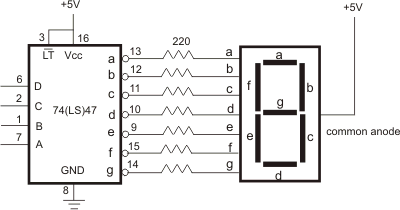
\includegraphics[scale=1.0]{images/DisplayResistors.png}
    \caption{Resistencias limitadoras de corriente}
    \label{Fig:Currentlimitingresistors}
\end{figure}

\pagebreak

\section{Resultados esperados}
\subsection{Funcionamiento completo}
Se requiere que al interconectar todos los circuitos el usuario interactúe con la entrada del \emph{dip-switch} y así seleccione el índice del dígito del año, mientras
este número se muestra directamente en el display de 7 segmentos.

\subsection{Optimización de recursos}
Recuerde que a pesar de obtener funciones separadas para las salidas de los Mapas de Karnaugh, es posible reutilizar operaciones entre los circuitos de salida.
Por ejemplo, piense en el siguiente caso hipotético en el que las funciones de salida de los Mapas de K. quedaran así:
$$ x = \bar A B \bar C + \bar A \bar C + \bar A$$
$$ y = AB\bar C + \bar C + B $$
$$ z = AB + \bar A \bar C + \bar A $$
$$ w = ABC + A\bar B \bar C + B $$

En la función $x$ aparecen varias veces $\bar A$ y $\bar C$, por lo que solamente es necesario utilizar una compuerta lógica para negar cada variable de entrada. Asimismo,
la variable negada $\bar A$ de la función $x$ puede reutilizarse en el circuito de la función $z$, donde aparece de nuevo. Incluso, el mintérmino completo de $x$ $(\bar A \bar C)$
se repite también en $z$, por lo que se posible reutilizar la salida de esa operación completa de $x$ directamente en $z$. 


\section{Conclusiones}
El funcionamiento del selector de índice es muy utilizado en electrónica digital y sirve para trasladar o codificar información única
en base a un índice o número que indica qué operación realizar. Esta operación es parte fundamental del funcionamiento de un microprocesador,
incluso de la tecnología actual.

\vspace{14pt}

En realidad, lo que se acaba de construir es conocido como un \textbf{Multiplexor} (coloquialmente MUX).